Springheadをダウンロードしてから使えるようにするまでの流れを説明します.

\section{ダウンロード}

Springheadのウェブサイト\url{http://springhead.info/wiki/}からzipアーカイブをダウンロードできます.
\KLUDGE ただし,アーカイブの更新は必ずしも頻繁ではありません (よくないことですが) ので,最新のコードが入手できない可能性があります.
\KLUDGE 常に最新のコードを使用したい人は,次に説明するSubversionレポジトリからコードを入手してください.

\section{SVNから入手する}

SpringheadはSubversionを用いてバージョン管理を行っています.
\KLUDGE この文書の執筆時点でSpringheadのSubversionレポジトリは
\begin{align*}
\text{\url{http://springhead.info/spr2/Springhead2/trunk}}
\end{align*}
\KLUDGE です.
\KLUDGE レポジトリからのコードのダウンロードは任意のユーザが行えますが,
\KLUDGE コードをコミットするには開発者として登録されている必要があります.

\KLUDGE %Subversionによるコードの入手方法については\url{http://springhead.info/wiki/}にて解説されていますのでそちらを参照して下さい.

\section{開発環境}

Springheadは処理系非依存の思想のもとで開発されています.
\KLUDGE このため,原理的にはWindows, Max, Unixなどの多くの処理系で動作するはずです.
\KLUDGE しかしながら,ほとんどの開発メンバーがWindows上のVisual Studioを用いて開発を行っているため,それ以外の環境で問題無く動作する保証は残念ながらありません (多分動かないでしょう).
\KLUDGE したがって,現状ではユーザーにもWindows + Visual Studioという環境での使用を推奨します.
WindowsやVisual Studioのバージョンについては,Windows 7/8/10, Visual Studio 2015では問題なく動作します.

\section{ライブラリのビルド}
\label{libbuild}

\KLUDGE 以下では,Springheadを保存したディレクトリを\path{C:\Springhead2}と仮定して話を進めます.
Springheadを入手したら,まずライブラリをビルドします.
\KLUDGE ただし,サンプルプログラムをビルドする場合に限りここでの作業は不要です (ライブラリは自動的に作成されます).

\KLUDGE まず,Visual Studioで以下のソリューションファイルを開いて下さい.
\begin{align*}
\text{\path{C:\Springhead2\src\Springhead14.0.sln}}
\end{align*}

\begin{center}\framebox{\footnotesize{%
\begin{minipage}{0.9\hsize}
\KLUDGE 【補足】 ファイル名末尾の数字は Visual Studio のバージョン番号を示しています.
\KLUDGE ただし,Visual Studio 2010 より古いバージョンについてはメジャーバージョン番号のみです.
\KLUDGE その他のソリューションファイル,プロジェクトファイルも同様の規則でナンバリングしてあります.
Visual Studio 2013 より以前の Visual Studio を使用する場合には適宜読み替えてください.
\end{minipage}
}}\end{center}


\begin{figure}[t]
\begin{center}
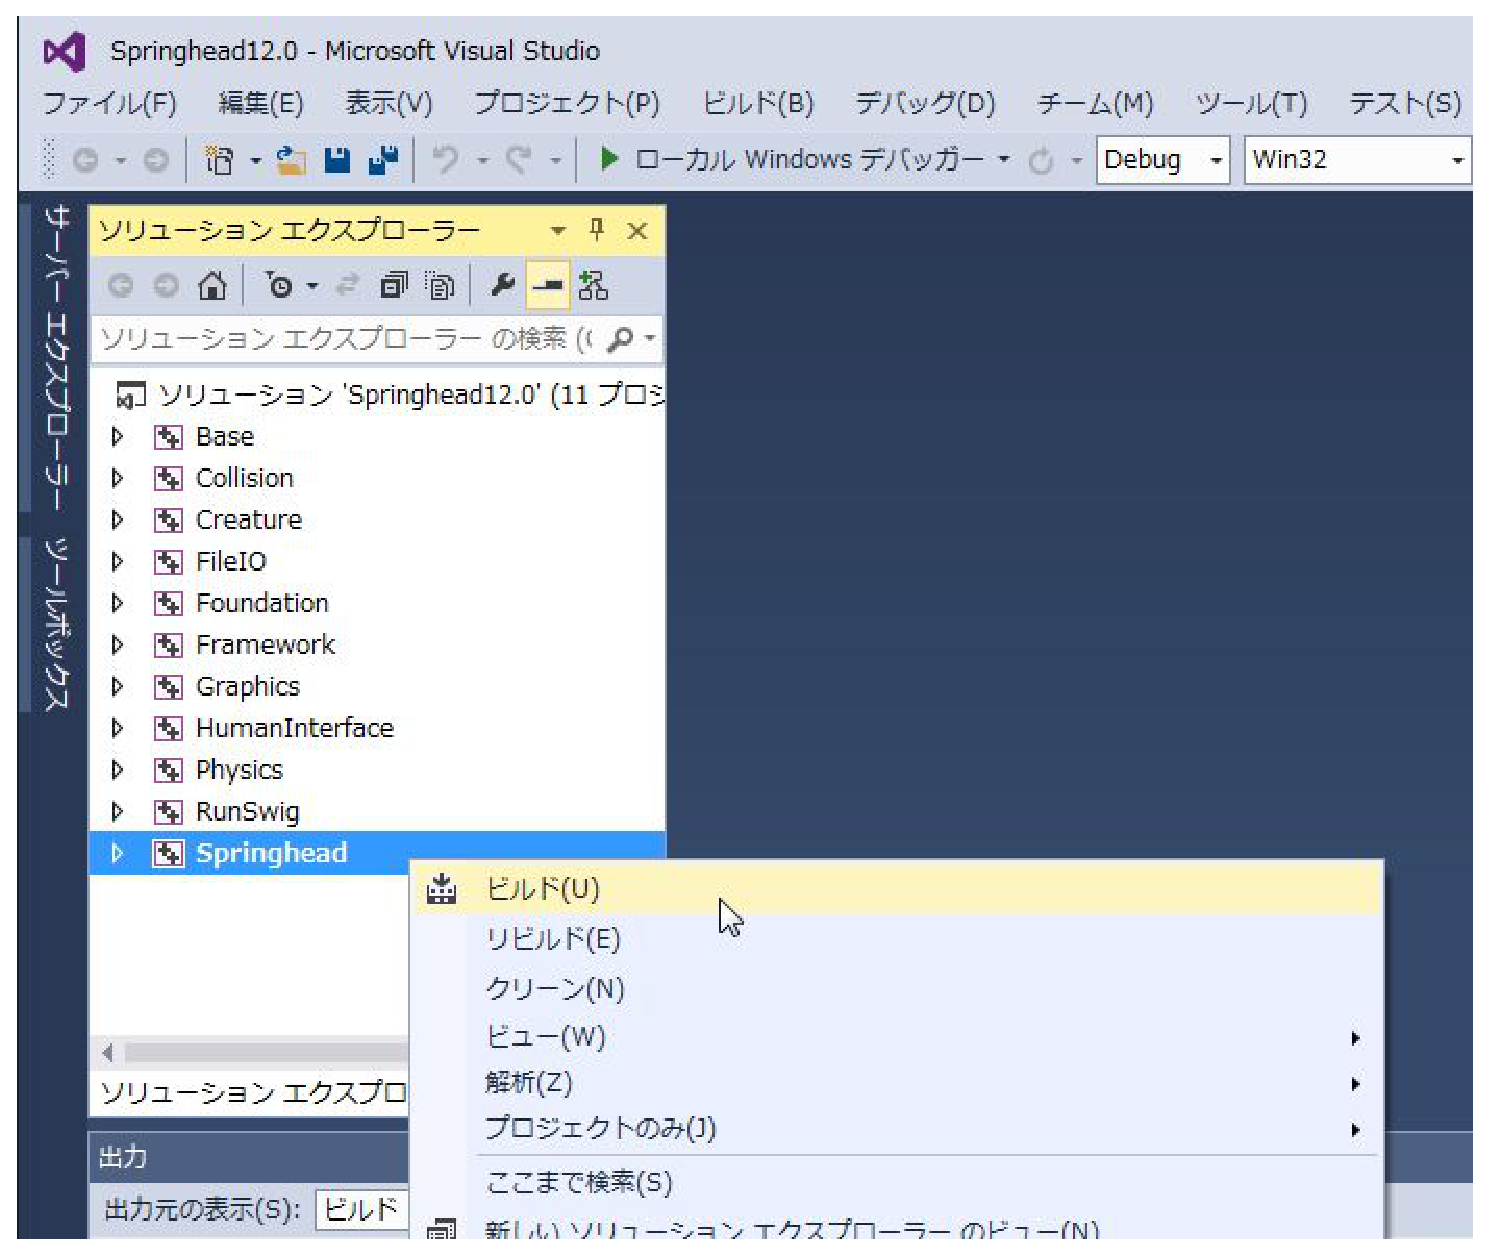
\includegraphics[width=.6\hsize]{fig/libbuild.eps}
\end{center}
\caption{Building the library}
\label{fig_libbuild}
\end{figure}
\KLUDGE ソリューションを開いたらFig.\,\ref{fig_libbuild}に示すように\url{Springhead}プロジェクトをビルドしてください.
\KLUDGE ビルドに成功したら\path{C:\Springhead2\lib\win32\}または\path{C:\Springhead2\lib\win64\}ディレクトリにライブラリファイルが作成されるはずです.

Table\,\ref{table_solution_config} に示すように,ビルドの設定ごとに異なるいくつかの構成が用意されています.
\KLUDGE ユーザアプリケーションの都合に合わせて使い分けてください.

\begin{table}[t]
\caption{Build configurations}
\label{table_solution_config}
\begin{center}
\begin{tabular}{lll}
\toprule
\KLUDGE 構成名				& ビルド設定					& 作成されるライブラリファイル名	\\ \midrule
\url{Release}		& multithread, DLL				& \url{Springhead14.0\# \#.lib}	    \\
\url{Debug}			& multithread, Debug, DLL		& \url{Springhead14.0\# \#D.lib}	\\
\url{Trace}			& multithread, Debug, DLL		& \url{Springhead14.0\# \#T.lib}	\\ \bottomrule
\multicolumn{3}{l}
{\footnotesize{%
\vbox{\vbox to 1mm{}
      \hbox{・ \url{\# \#} はプラットフォームを表す \url{Win32} 又は \url{x86} となります.}
      \hbox{・ \url{Trace} 構成とは,フレームポインタ情報付き \url{Release} 構成のことです.}}}}
\end{tabular}
\end{center}
\end{table}

\begin{center}\framebox{\footnotesize{%
\begin{minipage}{0.9\hsize}
\KLUDGE 【補足】 ライブラリファイルのビルド設定及び名称はこれまでの開発経緯による理由で,少々複雑になっています.
\begin{itemize}
\item{Visual Studio 2008 では,すべての構成が Static Link 設定です.}
\item{Visual Studio 2010 では, \url{Release} / \url{Debug} 構成が Static Link 設定,
\url{ReleaseDll} / \url{DebugDll} / \url{Trace} 構成が DLL 設定です.}
\item{Visual Studio 2012 では,すべての構成が DLL 設定です.}
\item{Visual Studio 2010 以前のバージョンでは,プラットフォームが 32ビットの場合,ライブラリファイル名に \url{Win32} が付きません.}
\item{Visual Studio 2010 の \url{ReleaseDll} 構成及び \url{DebugDll} 構成では,\url{.lib} の前にそれぞれ
\url{M} 及び \url{MD} が付きます.}
\end{itemize}
\end{minipage}
}}\end{center}


\section{サンプルプログラムのビルド}

\KLUDGE サンプルプログラムをビルドするには
\begin{align*}
\text{\path{C:\Springhead2\src\Samples\All14.0.sln}}
\end{align*}
\KLUDGE を開きます.
\KLUDGE ビルドしたいサンプルをスタートアッププロジェクトに設定し,ビルド,実行してください.

\KLUDGE 残念なことですが,すべてのサンプルプログラムが問題なく動作する状態には維持されていません.
\url{Physics/BoxStack}や\url{Physics/Joints}が比較的良くメンテナンスされていますので試してみてください.

\KLUDGE 実行時にDLLが見つからないためにエラーが起こるかもしれません。
\begin{align*}
\text{\path{Springhead2\bin\win32}}
\text{\path{Springhead2\bin\win64}}
\end{align*}
\KLUDGE にPathを通してください。

\section{アプリケーションの作成}
\label{sec_create_application}

\begin{figure}[t]
\begin{center}
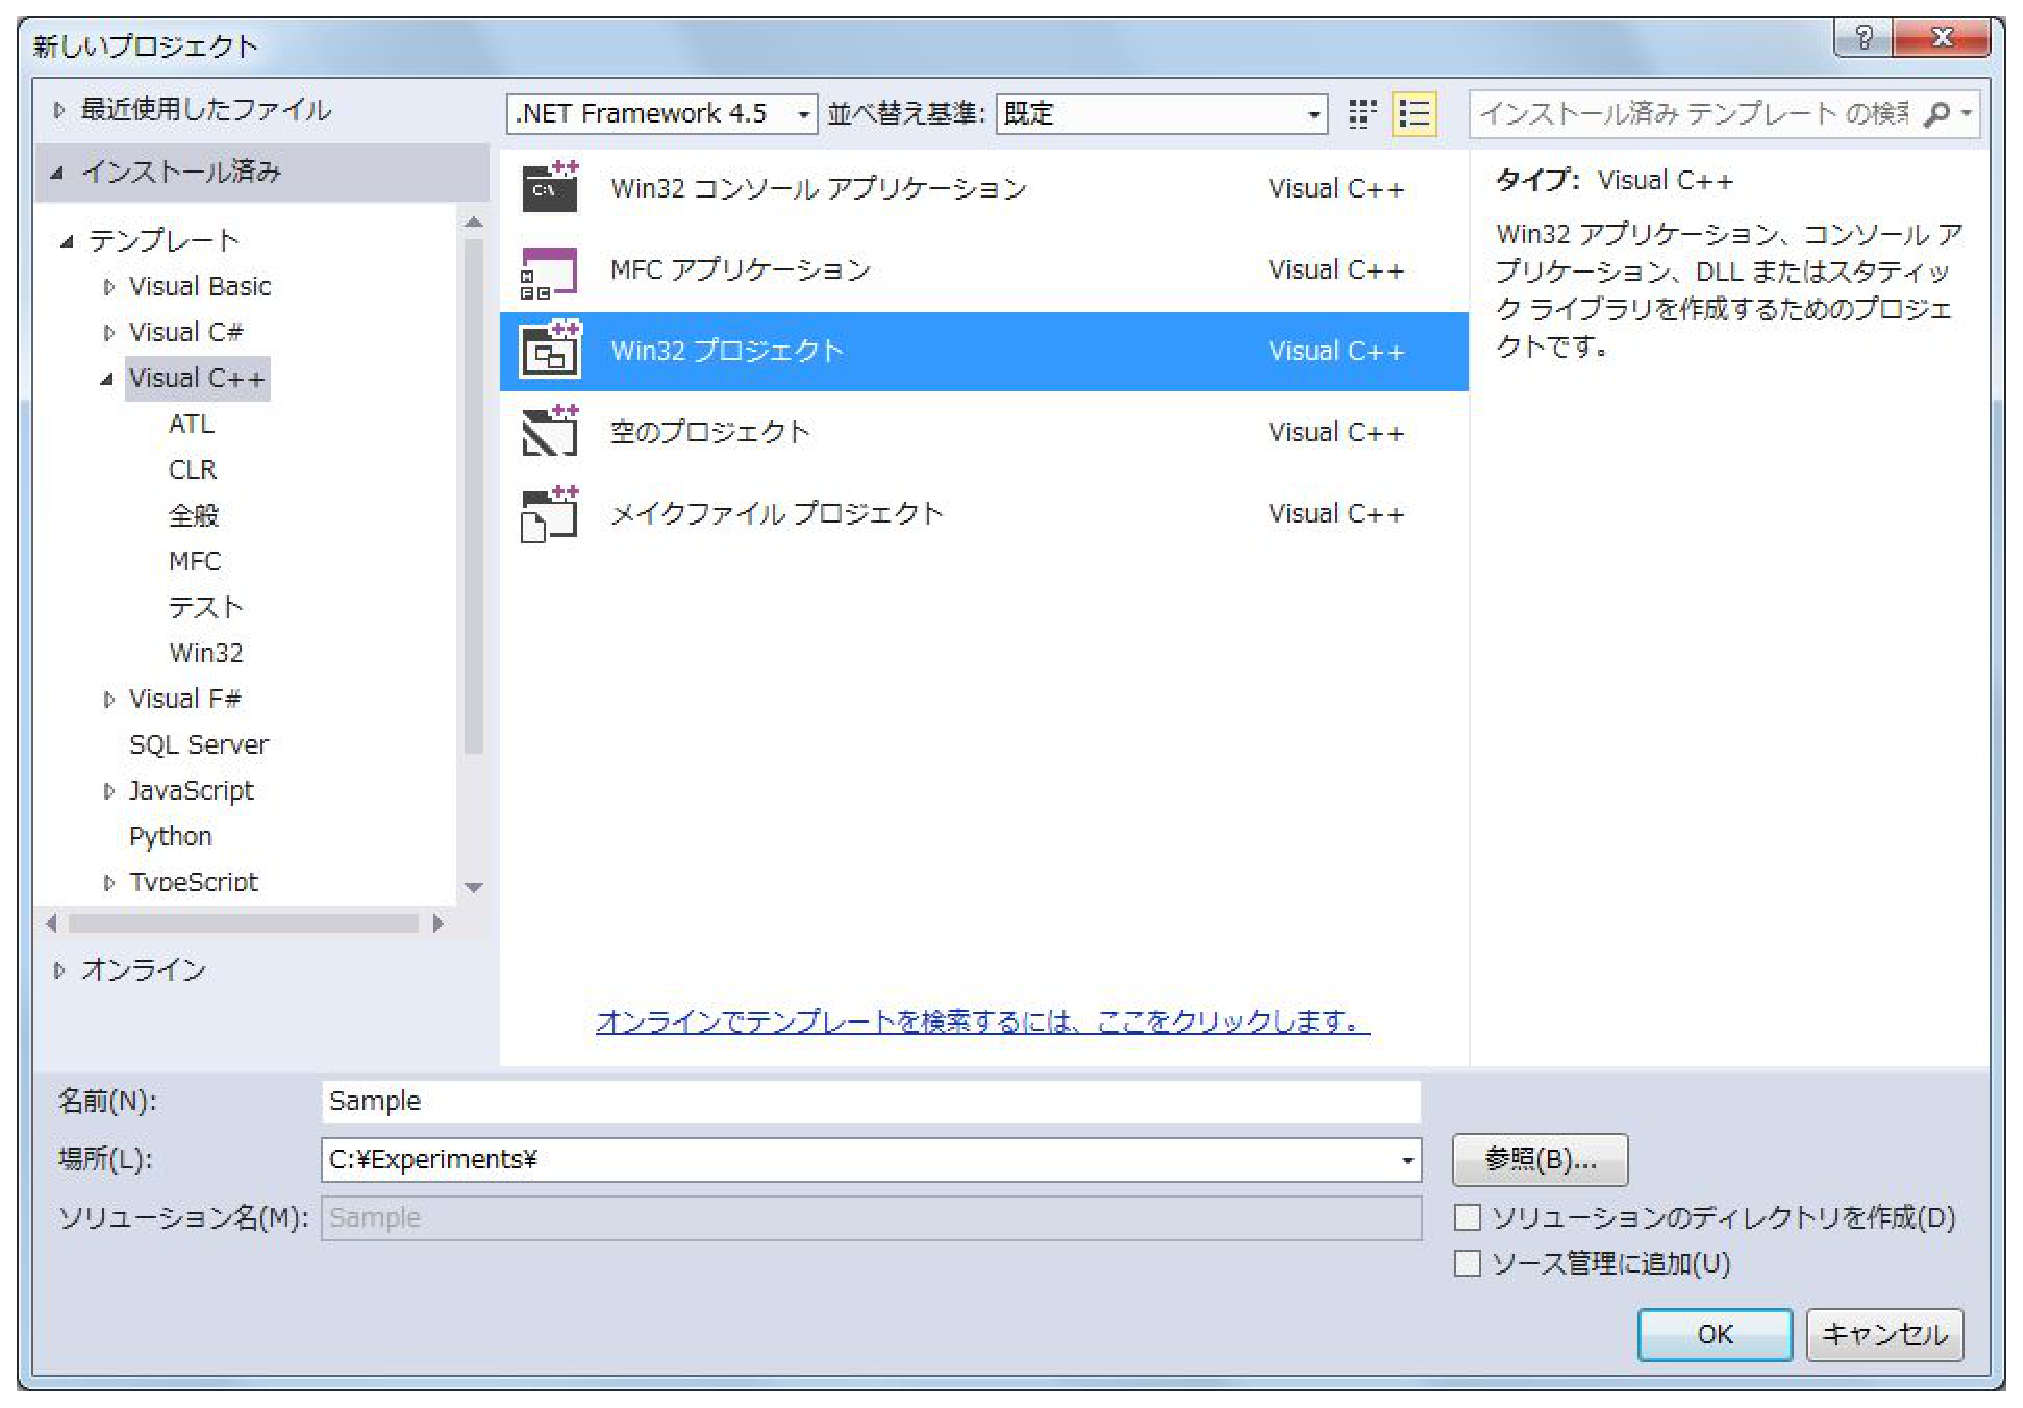
\includegraphics[width=.6\hsize]{fig/newproject1.eps}
\end{center}
\caption{Create new project}
\label{fig_newproject1}
\end{figure}

\begin{figure}[t]
\begin{center}
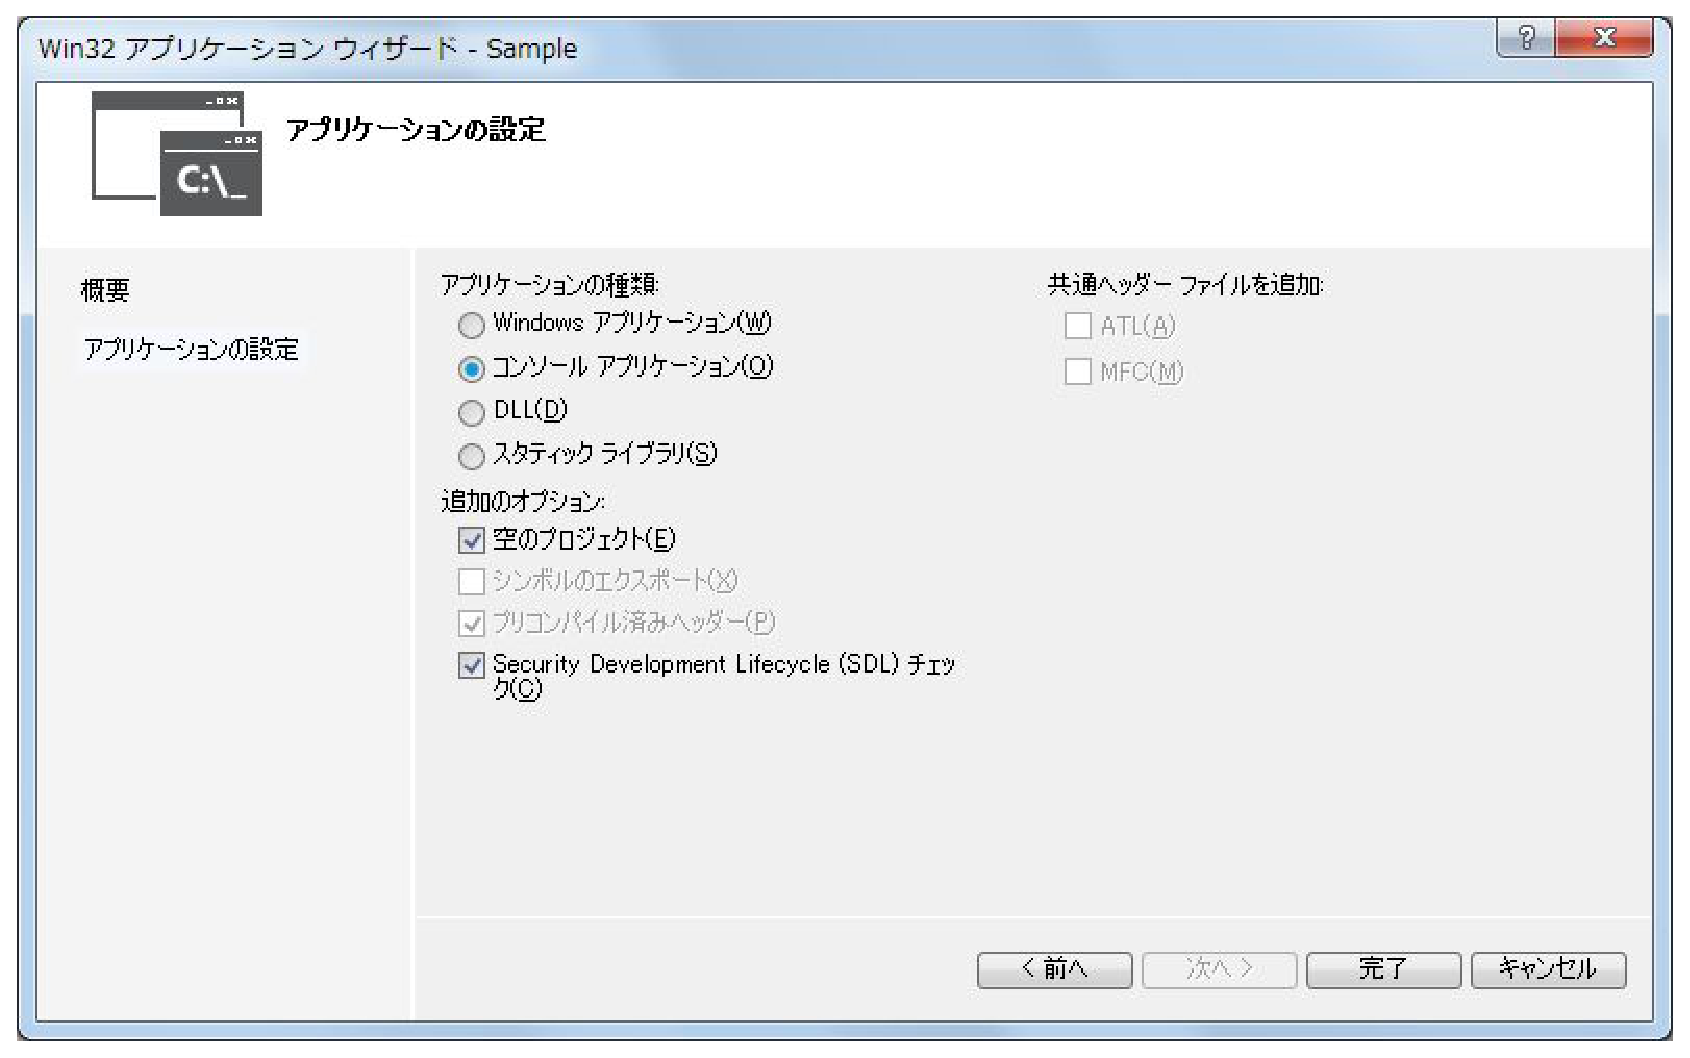
\includegraphics[width=.6\hsize]{fig/newproject2.eps}
\end{center}
\caption{Project configuration}
\label{fig_newproject2}
\end{figure}

\begin{figure}[t]
\begin{center}
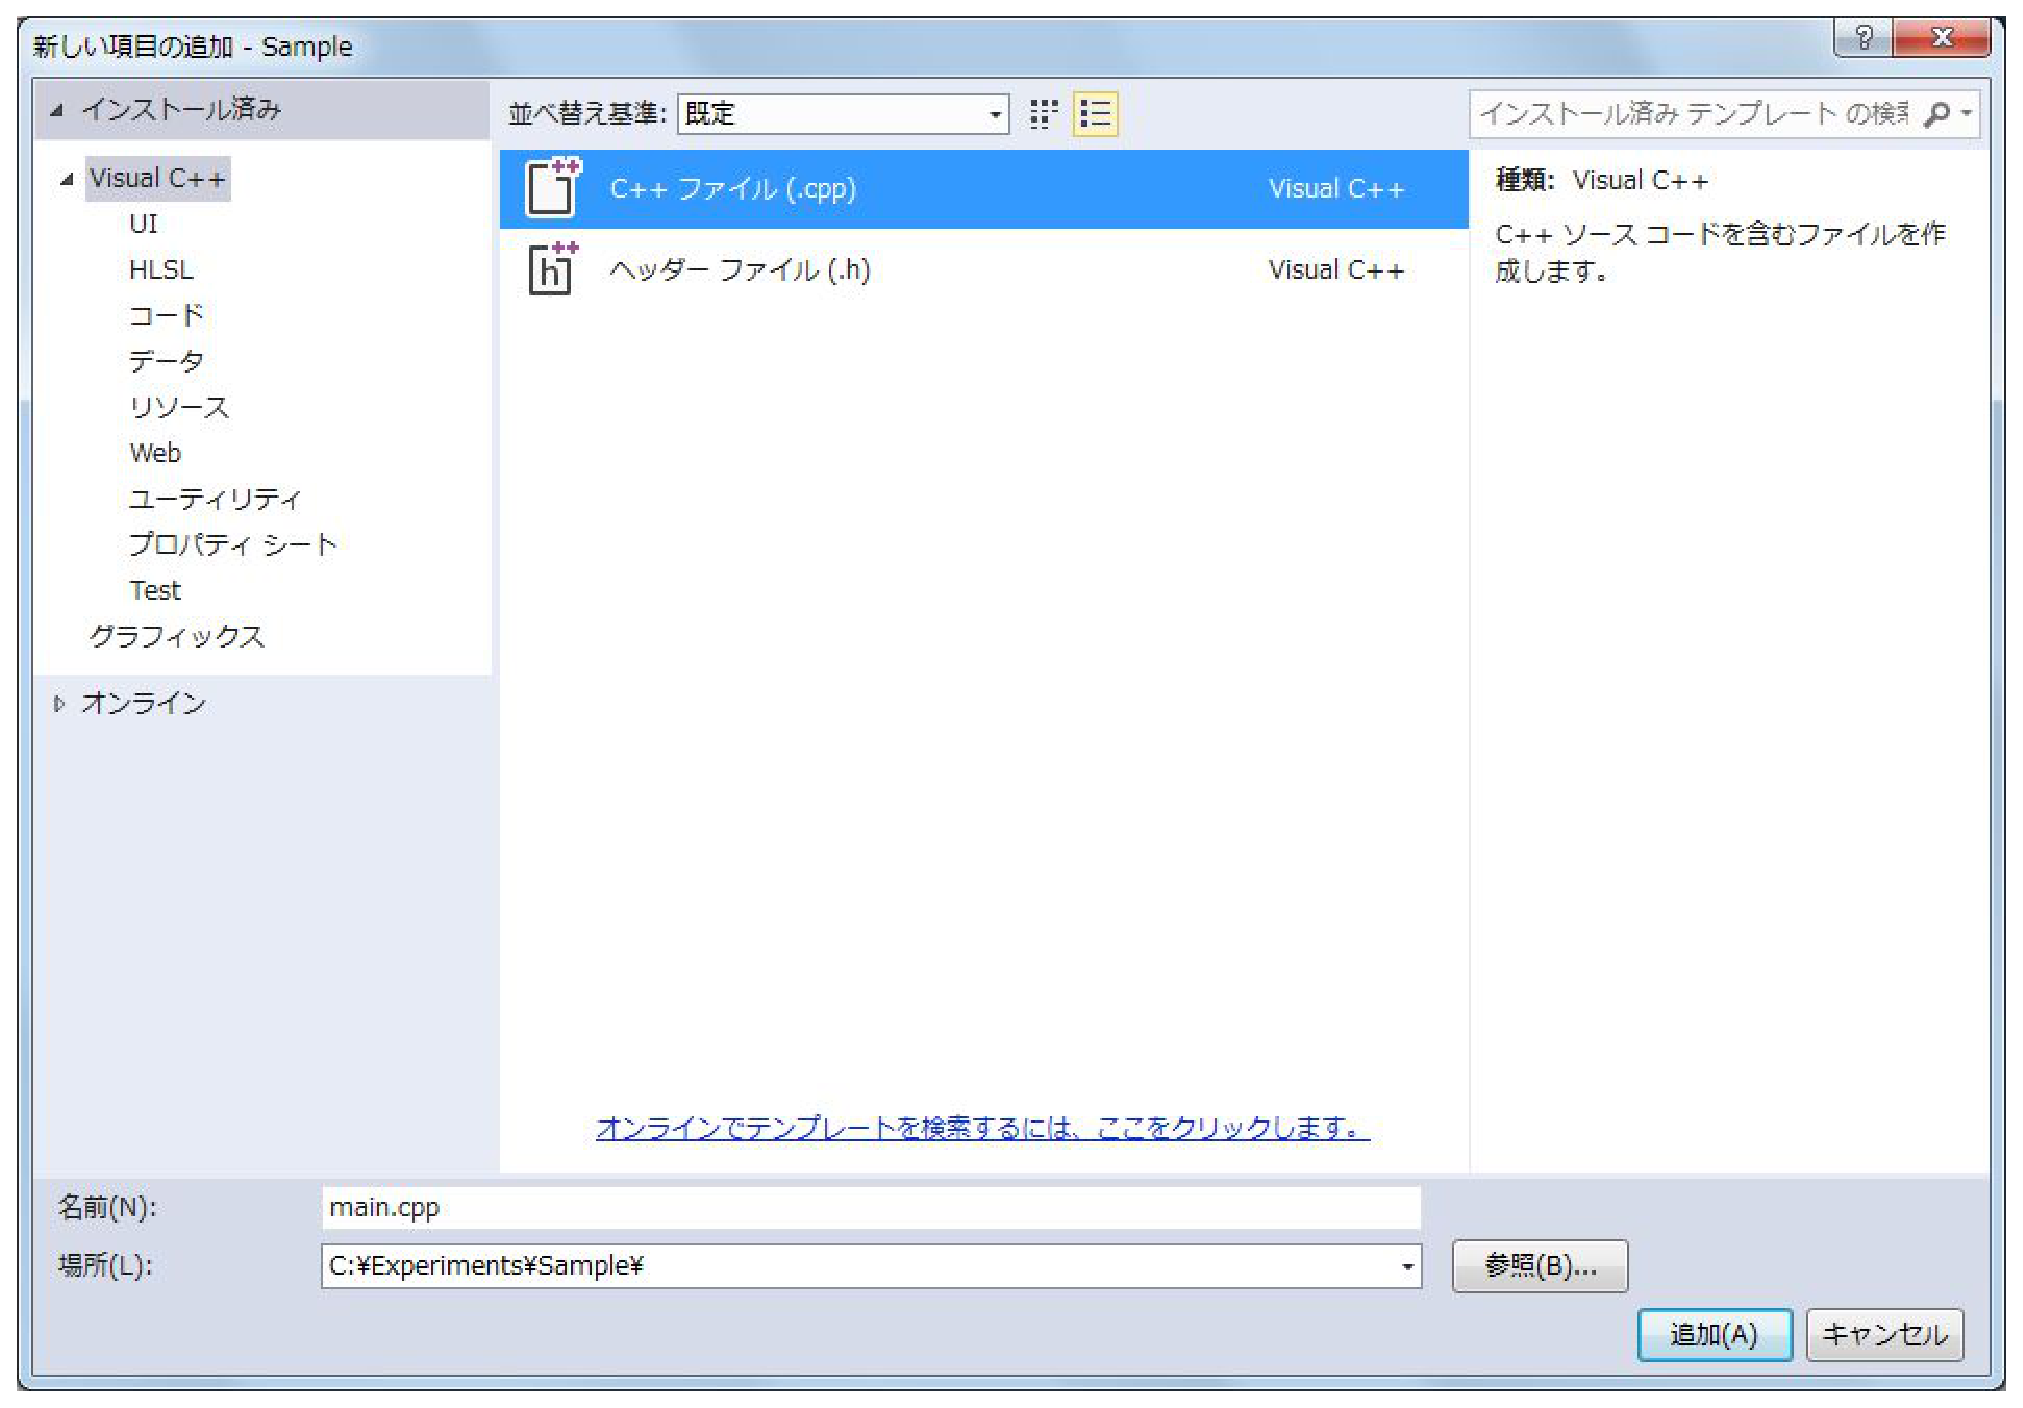
\includegraphics[width=.6\hsize]{fig/newproject3.eps}
\end{center}
\caption{Create source file}
\label{fig_newproject3}
\end{figure}

Springheadを使って簡単なアプリケーションプログラムを作成する道筋を説明します.
\KLUDGE 以下ではVisual Studio 2013を想定します.

\subsection*{プロジェクトの作成}

\KLUDGE 「Visual C++ Win32プロジェクト」を作成します.作成するディレクトリを \path{C:\Experiments} と仮定します. 他のディレクトリに作成する場合には,プロジェクトに指定するインクルードファイル及びライブラリファイルのパスが,保存した Springhead を正しく参照するように注意してください. プロジェクト名は好きな名前を付けてください.アプリケーションの設定で「コンソールアプリケーション」を選び,空のプロジェクトをチェックします.

\KLUDGE プロジェクトを作成したら「プロジェクト $>$ 新しい項目の追加 $>$ C++ファイル(.cpp)」としてソースファイルを作成します.
\KLUDGE ここでは仮に\url{main.cpp}とします.

\subsection*{ソースコードの編集}

\begin{table}[t]
\caption{Simplest program code}
\label{table_simplest_code}
{\small
\begin{sourcecode}
#include <Springhead.h>
#include <Framework/SprFWApp.h>
using namespace Spr;

class MyApp : public FWApp{
public:
    virtual void Init(int argc = 0, char* argv[] = 0){
        FWApp::Init(argc, argv);

        PHSdkIf* phSdk = GetSdk()->GetPHSdk();
        PHSceneIf* phscene = GetSdk()->GetScene()->GetPHScene();
        CDBoxDesc bd;
        
        // 床を作成
        PHSolidIf* floor = phscene->CreateSolid();
        floor->SetDynamical(false);
        bd.boxsize = Vec3f(5.0f, 1.0f, 5.0f);
        floor->AddShape(phSdk->CreateShape(bd));
        floor->SetFramePosition(Vec3d(0, -1.0, 0));
    
        // 箱を作成
        PHSolidIf* box = phscene->CreateSolid();
        bd.boxsize = Vec3f(0.2f, 0.2f, 0.2f);
        box->AddShape(phSdk->CreateShape(bd));
        box->SetFramePosition(Vec3d(0.0, 1.0, 0.0));

        GetSdk()->SetDebugMode(true);
    }
} app;

int main(int argc, char* argv[]){
    app.Init(argc, argv);
    app.StartMainLoop();
    return 0;
}
\end{sourcecode}
}
\end{table}

\KLUDGE 作成した\url{main.cpp}にTable\,\ref{table_simplest_code}に示すコードを書き込んでください.これがSpringheadを使用した (ほぼ) 最小のプログラムコードです.

\section*{プロジェクト設定}

\begin{figure}[t]
\begin{center}
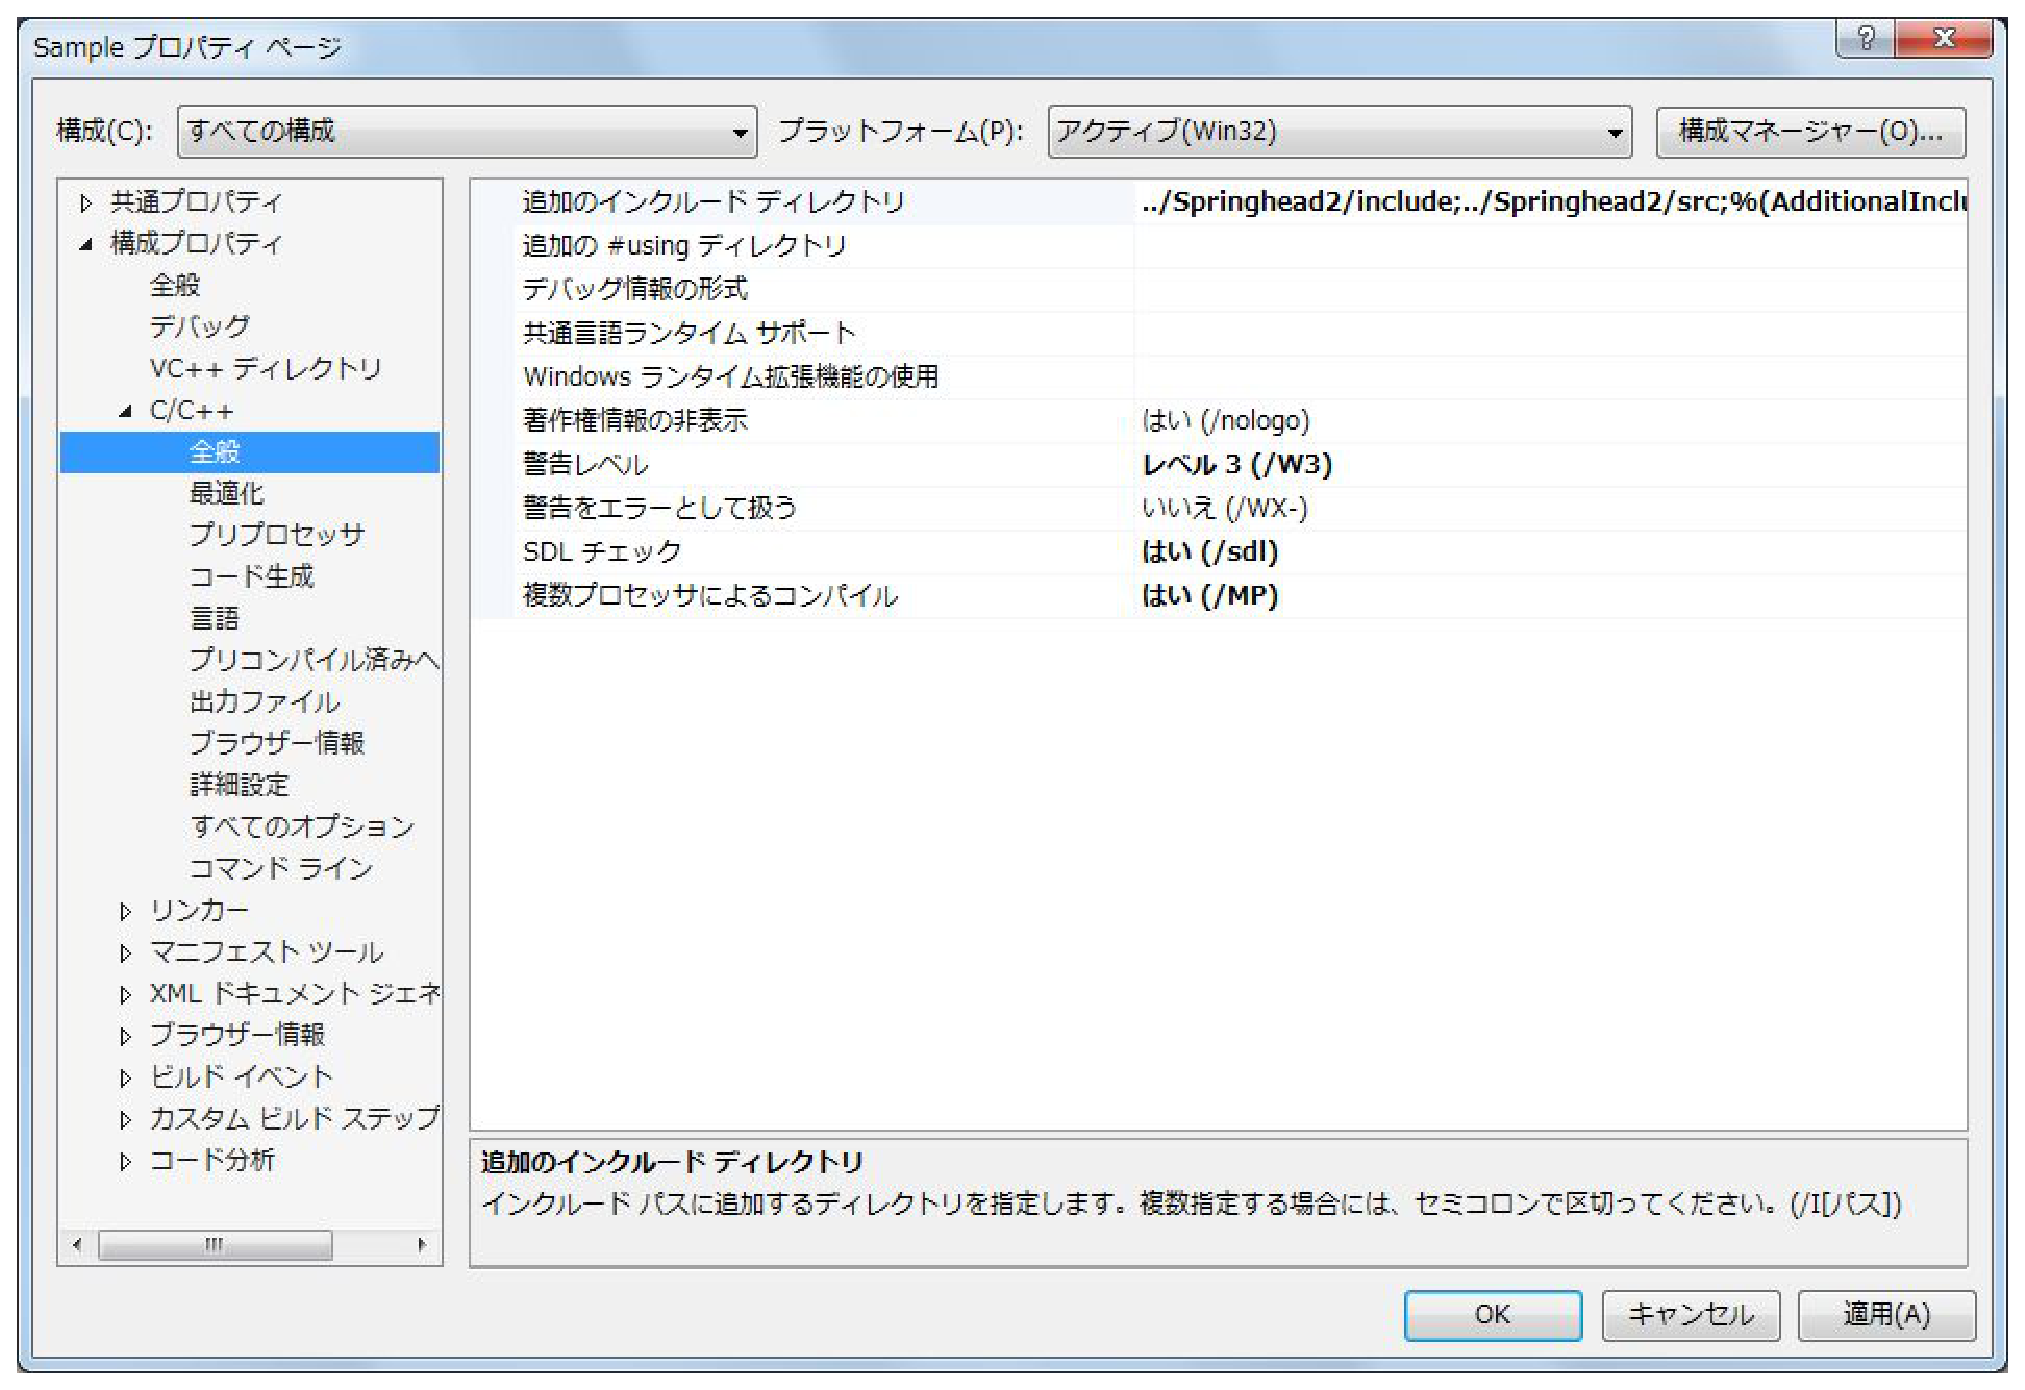
\includegraphics[width=.6\hsize]{fig/newproject4.eps}
\end{center}
\caption{Add include path}
\label{fig_newproject4}
\end{figure}

\begin{figure}[t]
\begin{center}
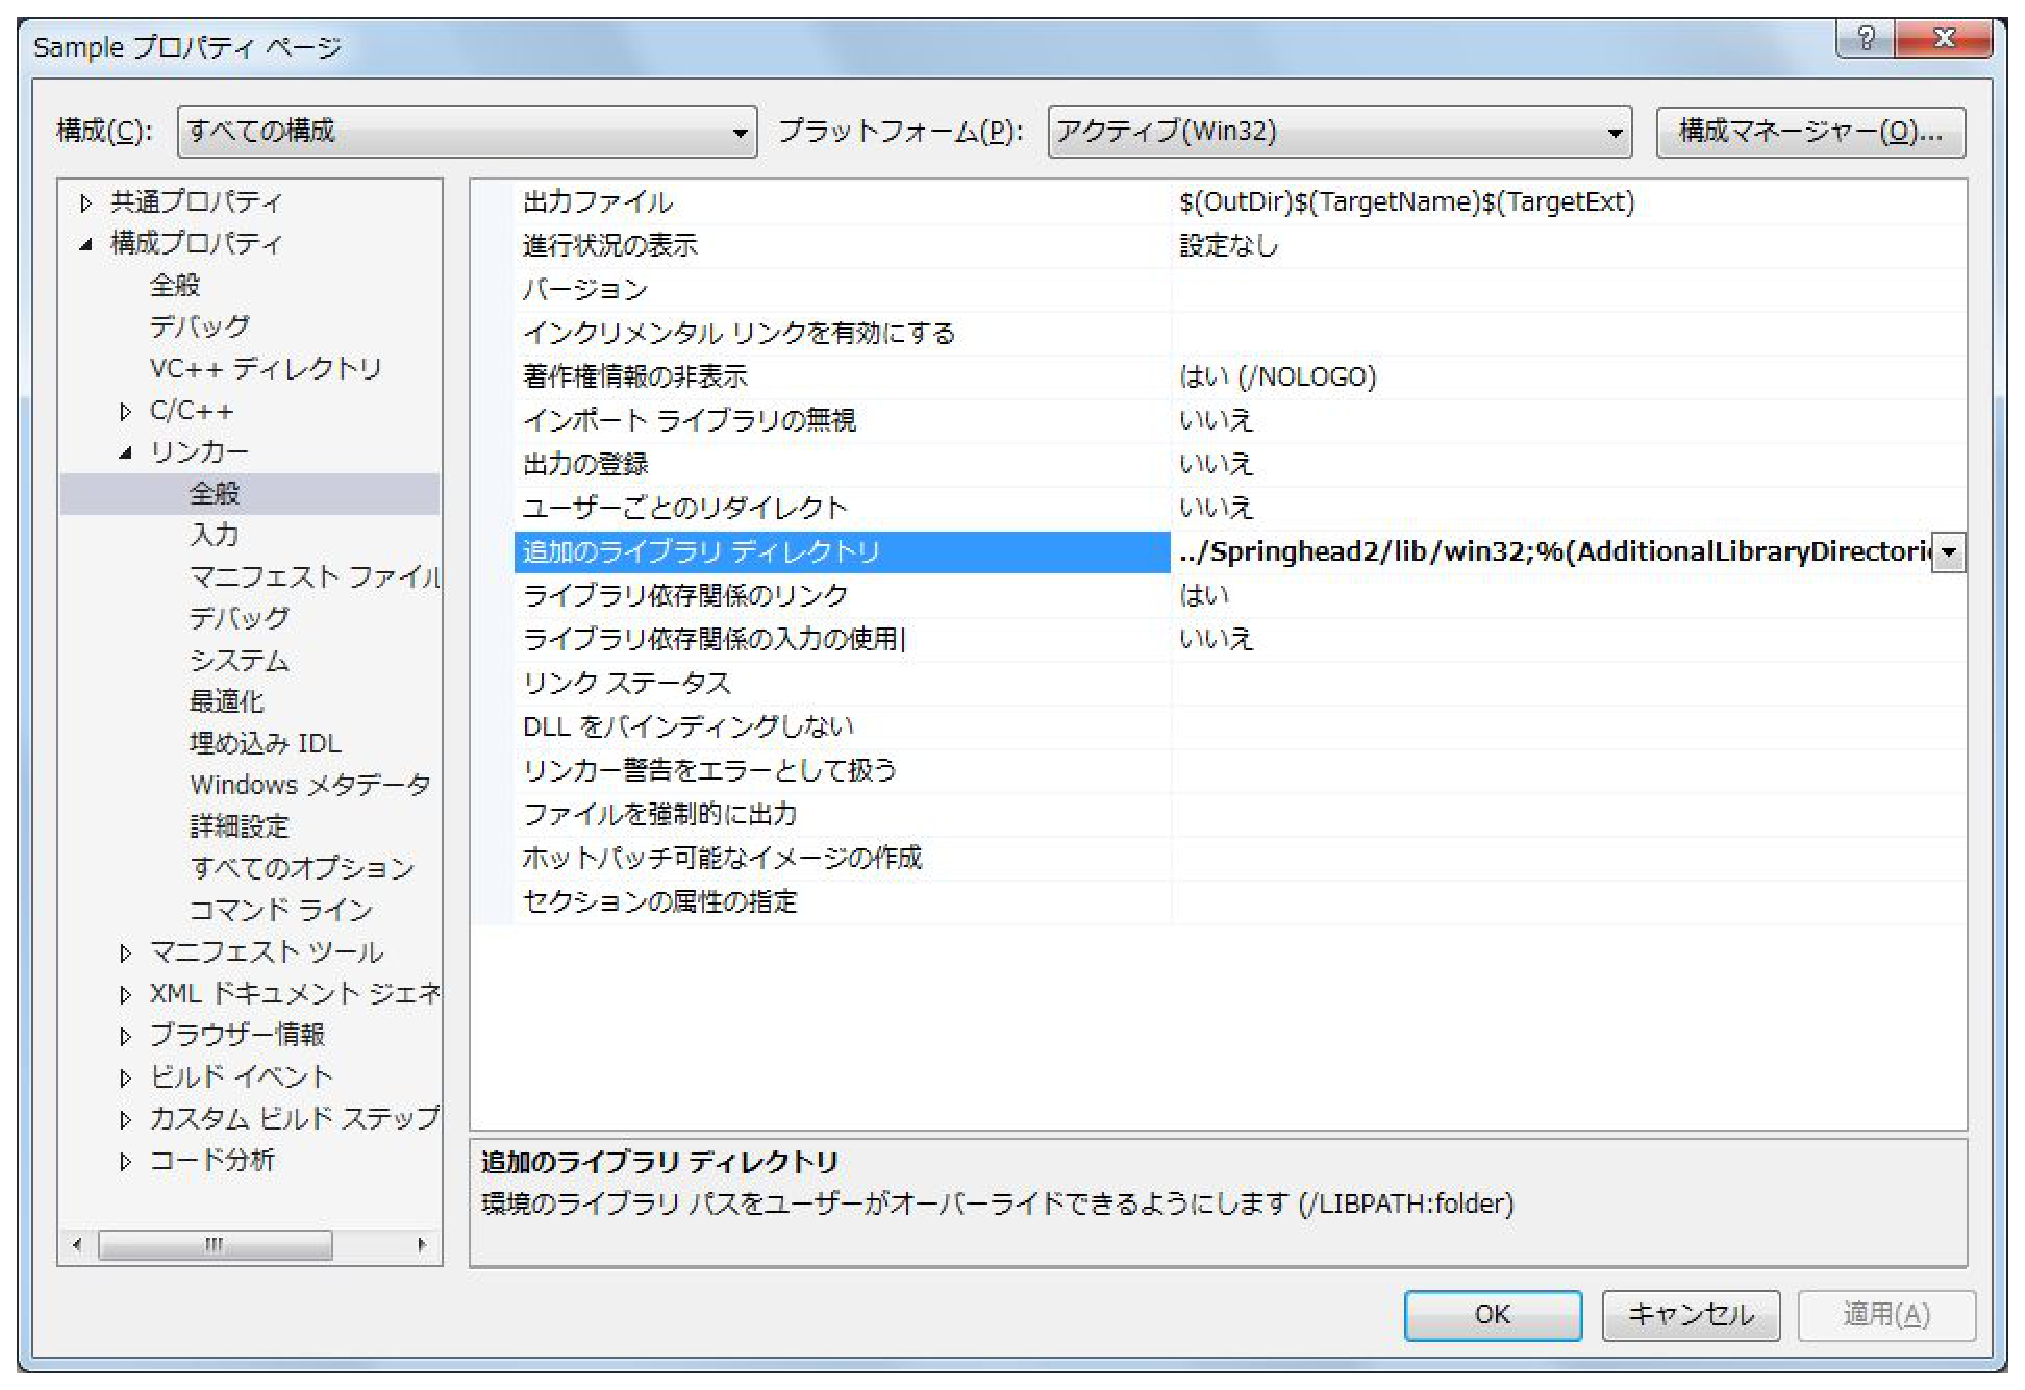
\includegraphics[width=.6\hsize]{fig/newproject5.eps}
\end{center}
\caption{Add library path}
\label{fig_newproject5}
\end{figure}

\begin{figure}[t]
\begin{center}
\begin{tabular}{c}
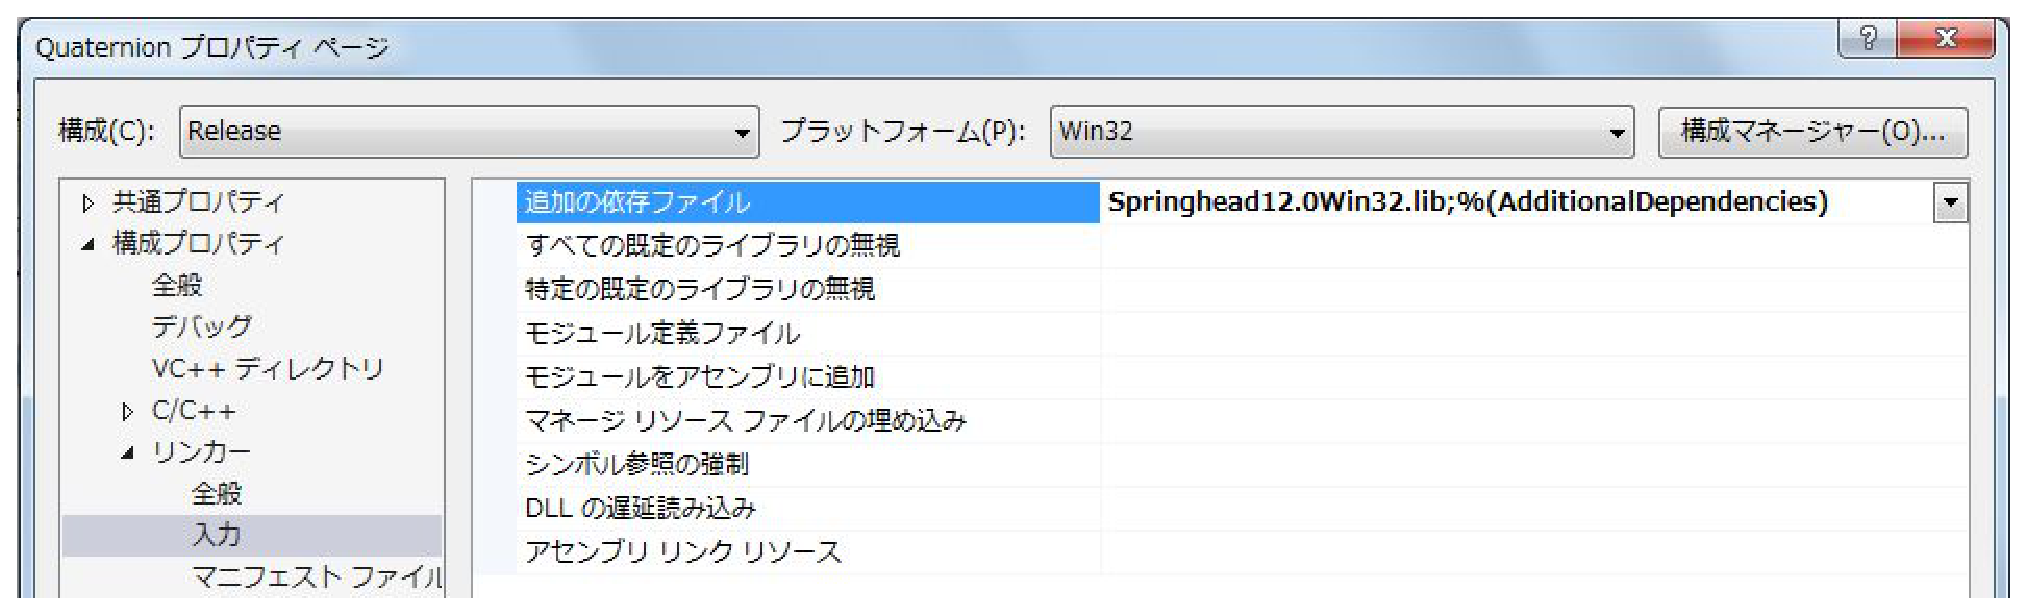
\includegraphics[width=.6\hsize]{fig/newproject6_truncate.eps} \\
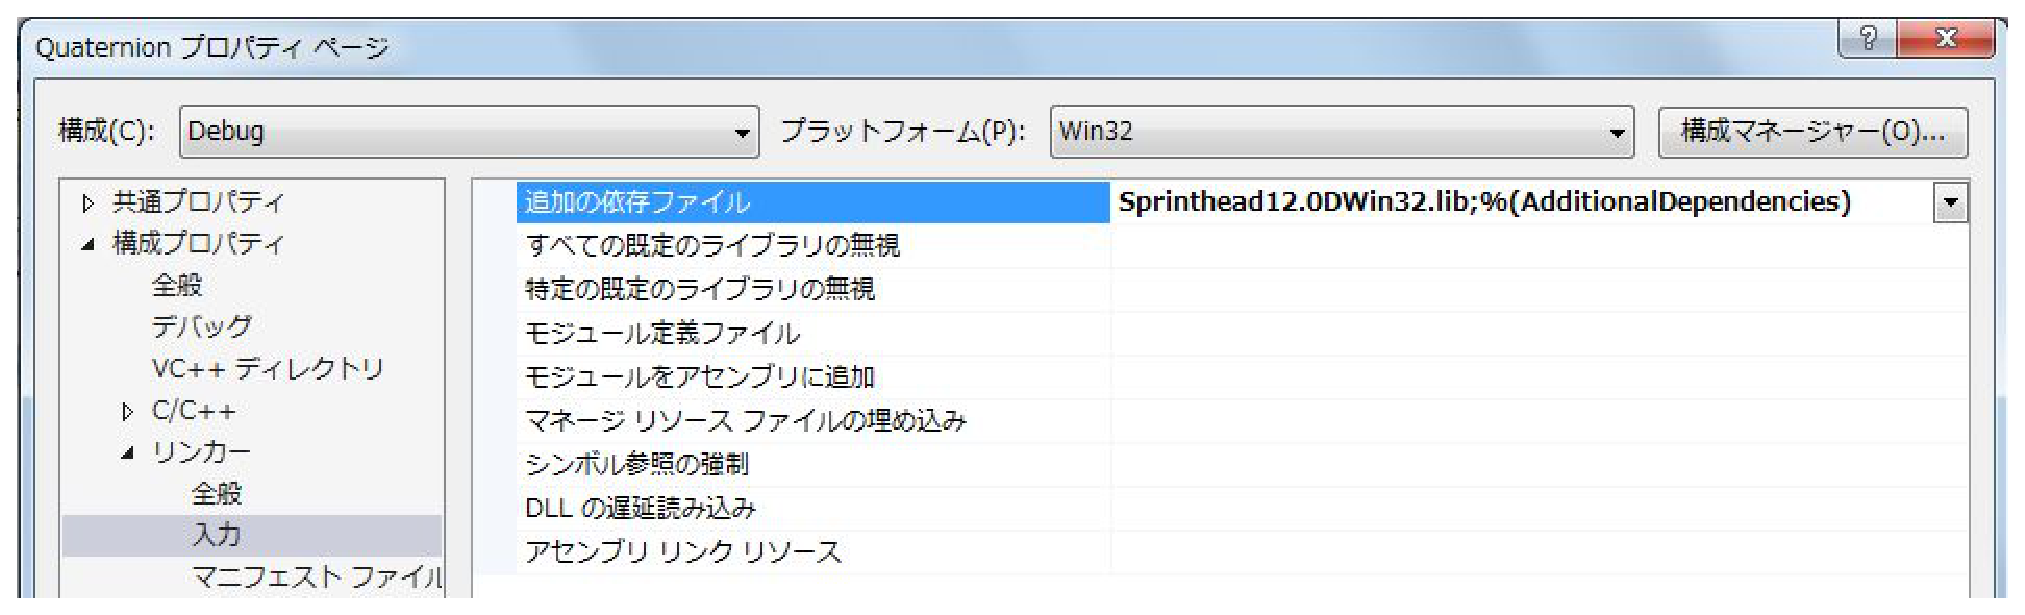
\includegraphics[width=.6\hsize]{fig/newproject7_truncate.eps}
\end{tabular}
\end{center}
\caption{Specify library file}
\label{fig_newproject6}
\end{figure}

\begin{figure}[t]
\begin{center}
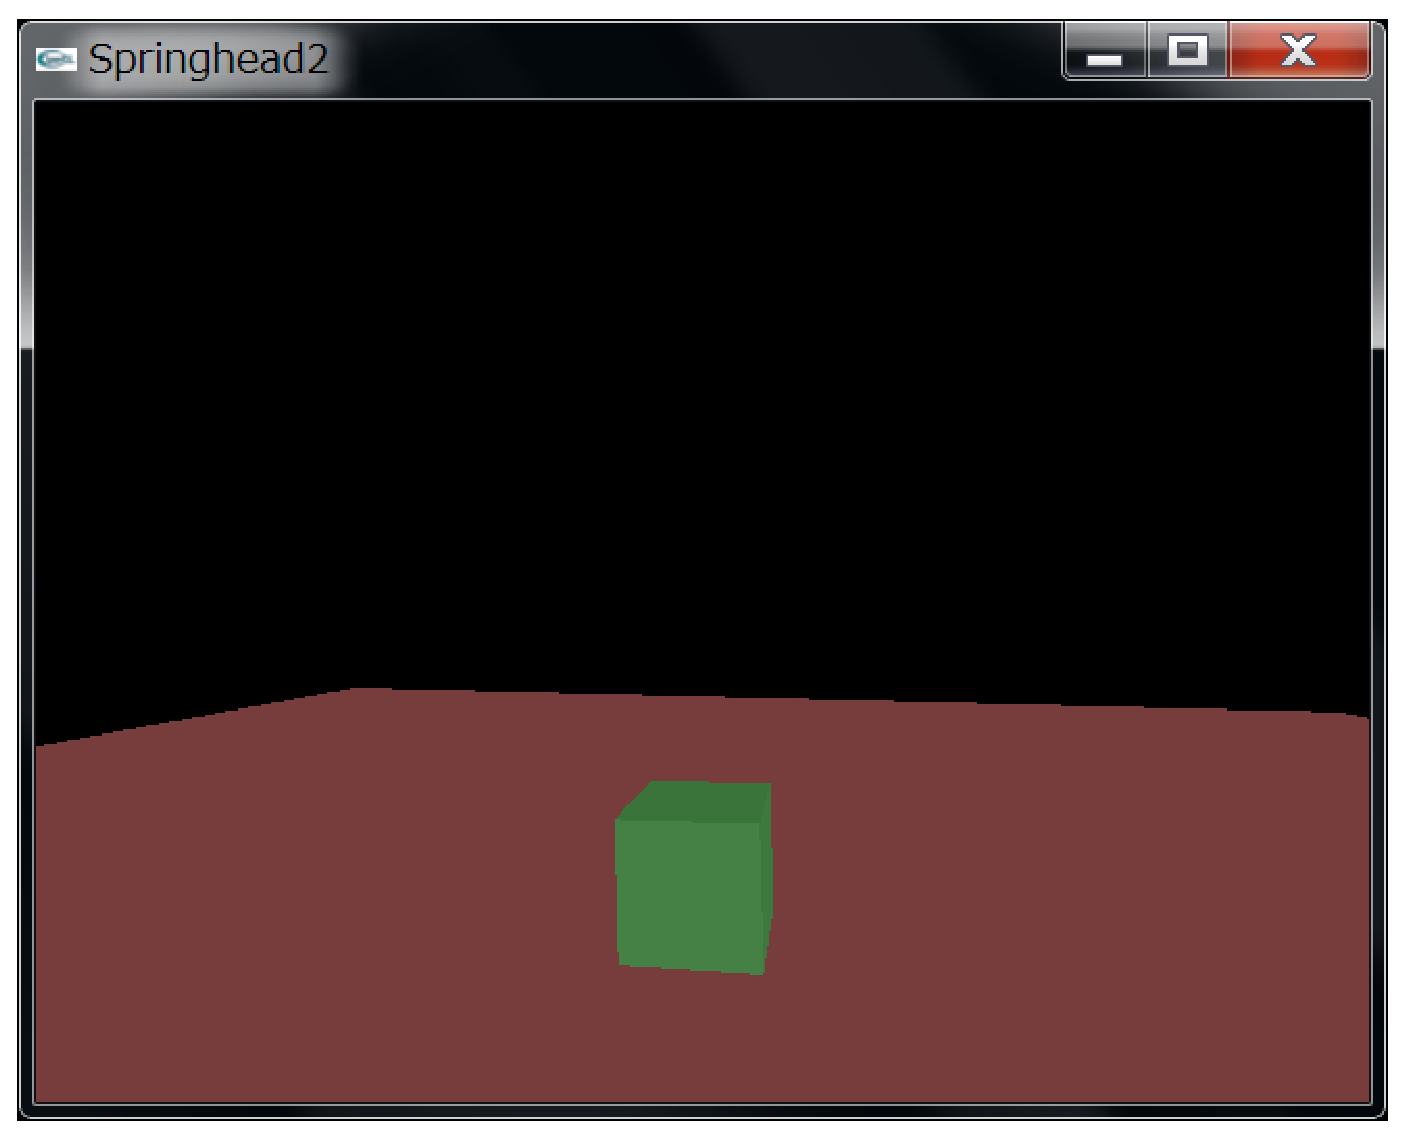
\includegraphics[width=.6\hsize]{fig/newproject8.eps}
\end{center}
\caption{Program running}
\label{fig_newproject8}
\end{figure}

\KLUDGE ビルドするまえにいくつかのプロジェクト設定が必要です.
64ビットプラットフォームを使用する場合には,プロパティーページの「構成マネージャー」で「\url{x64}」プラットフォームを新規作成して選択しておきます.
\KLUDGE また,\ref{libbuild} で説明したライブラリのビルドは済んでいるものとします.

\KLUDGE まずプロジェクトのプロパティページを開き,構成を「すべての構成」としてください.
\KLUDGE 次に「C/C++ $>$ 全般 $>$ 追加のインクルードディレクトリ」に,Fig.\,\ref{fig_newproject4}のようにSpringheadのインクルードファイルへのパスを指定してください.
\KLUDGE さらに,「リンカー $>$ 全般 $>$ 追加のライブラリディレクトリ」にFig.\,\ref{fig_newproject5}のようにSpringheadのライブラリファイルへのパスを指定します (64ビット構成ぼ場合は \url{win32} の代わりに \url{win64} を指定します).

\KLUDGE 今度は構成を「Debug」にします.
\KLUDGE 「C/C++ $>$ コード生成 $>$ ランタイムライブラリ」を「マルチスレッド デバッグ DLL (\url{/MDd})」にします.
\KLUDGE 次に「リンカー $>$ 入力 $>$ 追加の依存ファイル」に\url{Springhead14.0DWin32.lib}を追加してください.

\KLUDGE 最後に構成を「Release」に切り替えて同様の設定をします.
\KLUDGE ランタイムライブラリを「マルチスレッド DLL (\url{/MD})」として,追加の依存ファイルに\url{Springhead14.0Win32.lib}を追加します.

\section*{ビルド・実行}

\KLUDGE 以上で準備完了です.ビルド(F7)して,実行(F5)してみてください.
Fig.\,\ref{fig_newproject8}のような画面が出てくれば成功です.
